
\begin{figure}[H]
\caption{Overview of Payoffs by Treatment, Role, and Period}
\begin{center}
\includegraphics[width=0.8\textwidth]{Graphs/Structure.png}
\label{fig:structure}
	\begin{minipage}{0.75\textwidth}
	\footnotesize
	\vspace{3mm}
	{\it Note:} 100 Taler translate to 1 Euro.\\
	In the simple task, principals receive 5 Taler for each correctly positioned slider. In the creative task, principals receive 5 Taler for each per valid answer, 5 Taler for each new category, and  5 (10) Taler for each (very) original answer.\\
	Agents earn an additional 5 Taler each time that they press the time-out button. 
	\end{minipage}
\end{center}
\end{figure}


\newpage

\begin{figure}[H]
\caption{Screenshot of the Slider Task}
\begin{center}
\includegraphics[width=0.8\textwidth]{Graphs/screenshot_slidertask2.png}
\label{fig:screenshot}
	\begin{minipage}{0.75\textwidth}
	\footnotesize
	\vspace{3mm}
	{\it Note:} The figure presents a screenshot of the slider task. The screen displays the remaining time and the number of correctly positioned sliders. The time-out button is displayed at the bottom of the screen.  
	\end{minipage}
\end{center}
\end{figure}

\pagebreak

\begin{figure}[H]
	\centering
	\caption{Difference in Performance between Periods 2 and 1 by Treatment and Task}
	\label{fig:Bar_Chart_Round_1_2}
	\subfloat{\includegraphics[width=0.45\textwidth]{Graphs/Figure4a_paired_final2.pdf}}	
	\qquad
	\subfloat{\includegraphics[width=0.45\textwidth]{Graphs/Figure4b_paired_final2.pdf}}\\
	\begin{minipage}{0.9\textwidth}
	\footnotesize
	{\it Note:} The bars show the difference in mean (unstandardized) performance between Period 2 and Period 1. The whiskers depict 90\% confidence intervals of paired t-tests. Note that the Y-axes are not comparable across tasks.
	\end{minipage}
\end{figure}





\newpage


\begin{figure}[H]
\caption{Effect Sizes for Positive and Negative Reward Decisions by the Principal}
\begin{center}
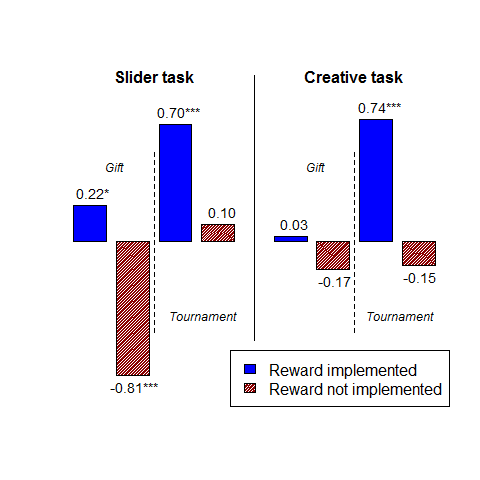
\includegraphics[width=0.75\textwidth]{Graphs/160308_Neg_Bonus_Dec.png}
\label{fig:Neg_Bonus_Dec}
	\begin{minipage}{0.8\textwidth}
	\footnotesize
	\vspace{5mm}
	{\it Note:} The dependent variable is standardized performance of agents in Period 2. The bars show the estimated regression coefficients of separate OLS regressions. Performance is measured as the number of correctly positioned sliders in the simple task and as the score achieved in the creative task. The regressions control for baseline performance in Period 1. The respective control group (slider or creative) serves as the reference category. Statistical significance: * p < 0.1, ** p < 0.05, *** p < 0.01. 
	\end{minipage}
\end{center}
\end{figure}

%-	Das sind 8 seprarate Regressionen, die immer die Kontrollgruppe enthält sowie entweder %die Agenten die von positiven oder negativen Bonusentscheidungen betroffen waren also:
%-	Gift positive Bonusentscheidung im Vergleich mit Kontrollgruppe Slider
%Gift negative Bonusentscheidung im Vergleich mit Kontrollgruppe Slider
%-	Turnier positive Bonusentscheidung im Vergleich mit Kontrollgruppe Slider
%Turnier negative Bonusentscheidung im Vergleich




\newpage
\begin{figure}[H]
\caption{Overview of Effect Sizes for All Gift Treatments}
\begin{center}
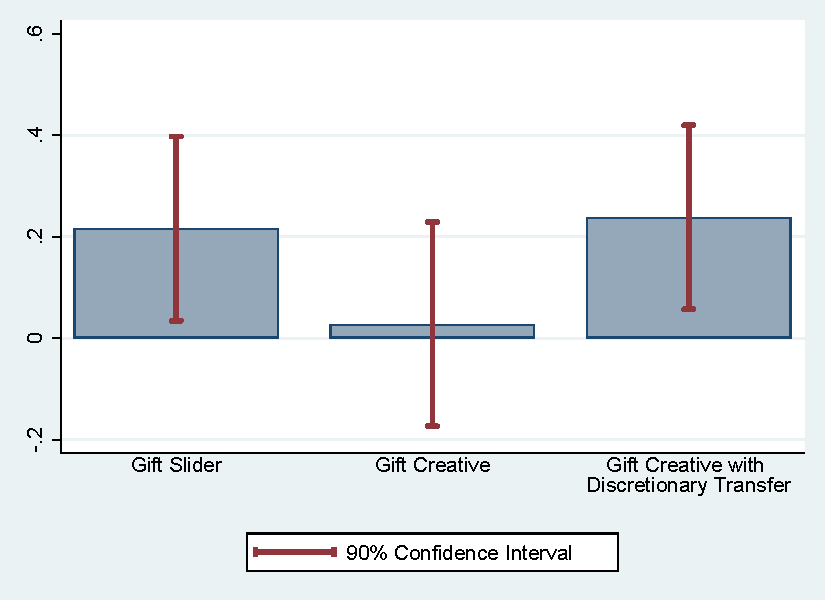
\includegraphics[width=0.75\textwidth]{Graphs/Figure5_new.pdf}
\label{fig:gift_treatments}
	\begin{minipage}{0.75\textwidth}
	\footnotesize
	\vspace{3mm}
	{\it Note:} The bars show the estimated regression coefficients of separate OLS regressions. Standardized performance (transfer) in Period 2 is the dependent variable. Performance is measured as the number of correctly positioned sliders in the simple  task,  as the score achieved in the creative task, and as the amount tranferred in the creative transfer treatments. The regression controls for baseline performance in Period 1. The respective control group serves as the reference category.
	\end{minipage}
\end{center}
\end{figure}



\newpage

\begin{figure}[H]
	\caption{Difference in Performance between Periods 3 and 1 by Treatment and Task}
	\label{fig:Bar_Chart_Round_1_3}
	\subfloat{\includegraphics[width=0.45\textwidth]{Graphs/Figure5a_paired_final3.pdf}}	
	\qquad
	\subfloat{\includegraphics[width=0.45\textwidth]{Graphs/Figure5b_paired_final3.pdf}}\\
	\begin{minipage}{0.9\textwidth}
	\footnotesize
	{\it Note:} The bars show the difference in mean performance between Period 3 and Period 1. The whiskers depict 90\% confidence intervals of paired t-tests. Note, this figure is on a bigger scale than Figure \ref{fig:Bar_Chart_Round_1_2} to improve readability.
	\end{minipage}
\end{figure}


\newpage